\documentclass[10pt]{article}
\usepackage[polish]{babel}
\usepackage[utf8]{inputenc}
\usepackage[T1]{fontenc}
\usepackage{amsmath}
\usepackage{amsfonts}
\usepackage{amssymb}
\usepackage[version=4]{mhchem}
\usepackage{stmaryrd}
\usepackage{graphicx}
\usepackage[export]{adjustbox}
\graphicspath{ {./images/} }

\title{XXXIV \\
 KORESPONDENCYJNY KURS Z MATEMATYKI }

\author{}
\date{}


\begin{document}
\maketitle
\section*{PRACA KONTROLNA nr 1}
październik 2004r.

\begin{enumerate}
  \item Staś kupił zeszyty 32 -kartkowe po 80 gr za sztukę i zeszyty 60 -kartkowe po $1,20 \mathrm{zł}$ za sztukę i zapłacił 13,20 zł. Ile zeszytów 60 -kartkowych kupił Staś, jeśli było ich więcej niż zeszytów 32-kartkowych?
  \item Rozwiązać nierówność
\end{enumerate}

$$
\frac{x^{2}+x}{x^{3}-x} \leqslant 1
$$

\begin{enumerate}
  \setcounter{enumi}{2}
  \item Dana jest parabola o równaniu $y=-x^{2}+2 x+3$. Znaleźć równanie paraboli, która jest symetryczna do danej względem punktu $S(2,1)$, oraz wyznaczyć punkty, w których przecina ona osie układu współrzędnych. Sporządzić rysunek.
  \item W trójkącie prostokątnym równoramiennym $A B C$ dany jest wierzchołek kąta prostego $C(1,1)$, a bok $\overline{A B}$ leży na prostej $x+5 y+7=0$. Wyznaczyć współrzędne wierzchołków $A$ i $B$.
  \item W ostrosłupie prawidłowym sześciokątnym kąty płaskie ścian bocznych przy wierzchołku są równe $\alpha$. Wyznaczyć cosinus kąta między sąsiednimi ścianami bocznymi tego ostrosłupa.
  \item Dany jest trójkąt równoramienny o kącie przy podstawie $\alpha$ i ramieniu $b$. Ramiona tego trójkąta przecięto prostą odcinając z niego deltoid. Wyznaczyć kąty pozostałego mniejszego trójkąta oraz jego pole. Kiedy zadanie ma rozwiązanie?
  \item Rozwiązać nierówność
\end{enumerate}

$$
\sqrt{2^{x-2}+3} \leqslant 2^{x}-2
$$

\begin{enumerate}
  \setcounter{enumi}{7}
  \item Wyznaczyć dziedzinę oraz narysować wykres funkcji $s(x)$ danej wzorem
\end{enumerate}

$$
s(x)=\log _{2}\left(1-x+x^{2}-x^{3}+\ldots\right)
$$

Przy pomocy wykresu określić zbiór wartości tej funkcji.\\
9. Rozwiązać równanie

$$
\operatorname{tg} 3 x=\frac{\sin 4 x}{\cos 2 x}
$$

\section*{PRACA KONTROLNA nr 2}
\begin{enumerate}
  \item Liczby o $45 \%$ mniejsza i o $32 \%$ większa od ułamka okresowego 0,(60) są pierwiastkami trójmianu kwadratowego o współczynnikach całkowitych względnie pierwszych. Obliczyć resztę z dzielenia tego trójmianu przez dwumian $(x-1)$.
  \item Wykres funkcji $f:[0,5] \rightarrow R$ jest przedstawiony na rysunku obok. Narysować wykres funkcji $g(x)=f(x)-f(5-x)$ i zapisać ją wzorem.
  \item Obliczyć wartości $\sin \alpha$ i $\cos \alpha$, jeśli wiadomo, że\\
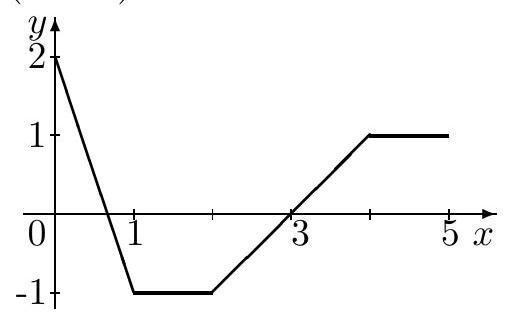
\includegraphics[max width=\textwidth, center]{2024_11_16_8518088a6e381b1443b2g-2}
\end{enumerate}

$$
\sin \alpha+3 \cos \alpha=\frac{1}{\cos \alpha}, \quad \alpha \in[0, \pi] \backslash\left\{\frac{\pi}{2}\right\} .
$$

\begin{enumerate}
  \setcounter{enumi}{3}
  \item Suma 20 pierwszych wyrazów pewnego ciągu arytmetycznego jest równa zeru, a iloczyn dziesiątego i jedenastego wyrazu wynosi -1 . Dla jakich liczb naturalnych $n$ suma $n$ pierwszych wyrazów tego ciągu przekracza 77 ?
  \item Trapez równoramienny jest wpisany w okrąg o promieniu $R$, a jedną z jego podstaw jest średnica tego okręgu. W trapez ten daje się wpisać okrąg. Wyznaczyć jego promień.
  \item Środek kuli opisanej na ostrosłupie prawidłowym trójkątnym leży w odległości $d$ ponad podstawą ostrosłupa, a kąt nachylenia krawędzi bocznej do podstawy wynosi $\alpha$. Obliczyć objętość ostrosłupa.
  \item Wyznaczyć wszystkie wartości parametru rzeczywistego $m$, dla których funkcja
\end{enumerate}

$$
f(x)=\frac{x+1}{x^{2}+m x+4}
$$

jest dodatnia i rosnąca na odcinku $(0,1)$.\\
8. Nie korzystając z rachunku różniczkowego wyznaczyć dziedzinę i zbiór wartości funkcji

$$
f(x)=\sqrt{\sqrt{2}-\cos x-\sqrt{3} \sin x}, x \in[0, \pi]
$$

\begin{enumerate}
  \setcounter{enumi}{8}
  \item Rozwiązać układ równań
\end{enumerate}

$$
\left\{\begin{array}{r}
|x+1| y=4 \\
x^{2}-4|x|+2 y-1=0
\end{array}\right. \text {. }
$$

Przedstawić ilustrację graficzną obu równań i zaznaczyć na rysunku znalezione rozwiązania.

\section*{PRACA KONTROLNA nr 3}
grudzień 2004r.

\begin{enumerate}
  \item W pewnej szkole zapytano uczniów klas maturalnych ile razy w ostatnim miesiącu ucze-\\
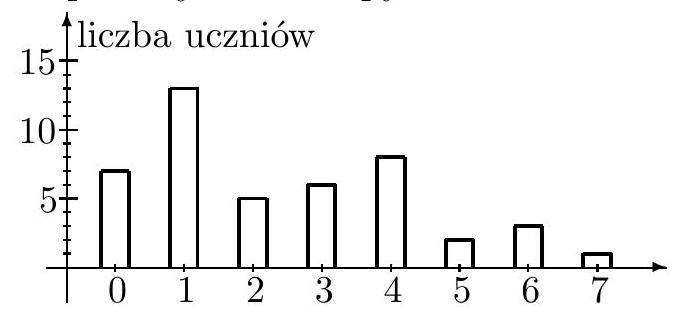
\includegraphics[max width=\textwidth, center]{2024_11_16_8518088a6e381b1443b2g-3(1)}\\
stniczyli w imprezie kulturalnej. Wyniki przedstawiono na diagramie obok. Obliczyć: a) Ilu uczniów jest w klasach maturalnych tej szkoły; b) Ile razy średnio w miesiącu uczeń był na imprezie kulturalnej. Sporządzić diagram kołowy przedstawiający procentowo otrzymane wyniki.
  \item Turysta zauważył, że w pewnym miejscu na odcinku 10 m potok górski płynie w korycie skalnym, które w przekroju pionowym tworzy trapez o dolnej podstawie 2 m i górnej 3 m . Wysokość koryta wynosi 50 cm , przy czym woda wypełnia koryto jedynie na głębokość 10 cm. Turysta ustalił również, że czas przepływu wody przez koryto wynosi 3 sekundy. Ile litrów wody przepływa przez ten potok w ciągu jednej sekundy?
  \item Wykazać, że dla dowolnych liczb dodatnich $a, b$ prawdziwa jest nierówność
\end{enumerate}

$$
(a+b)^{3} \leqslant 4\left(a^{3}+b^{3}\right)
$$

Wsk. Podzielić obie strony przez $b^{3}$ i wprowadzić jedną zmienną.\\
4. Boki $\overline{A B}$ i $\overline{A D}$ równoległoboku leżą odpowiednio na prostych $3 x+4 y-7=0$ i $x-2 y+1=0$. Wyznaczyć współrzędne wierzchołka $C$ tego równoległoboku wiedząc, że jego wysokość do boku $\overline{A B}$ wynosi 2 , a wierzchołek $B$ ma współrzędne $(5,-2)$.\\
5. W trójkącie ostrokątnym $A B C$ dane są bok $B C=\frac{5}{2} \sqrt{5} \mathrm{~cm}$ oraz wysokości $B D=\frac{11}{2} \mathrm{~cm}$ i $C E=5 \mathrm{~cm}$. Obliczyć obwód tego trójkąta oraz cosinus kąta $\angle B A C$.\\
6. Spośród dwudziestu najmniejszych, nieparzystych liczb naturalnych wylosowano (bez zwracania) dwie. Obliczyć prawdopodobieństwo, że otrzymano: a) dwie liczby pierwsze; b) dwie liczby względnie pierwsze.\\
7. Rozwiązać nierówność $\log _{2} x^{\log _{4} x} \geqslant \log _{x} 16$.\\
8. Niech $f(m)$ oznacza sumę trzecich potęg pierwiastków rzeczywistych równania kwadratowego $x^{2}+(m+3) x+m^{2}=0$ z parametrem $m$. Wyznaczyć wzór funkcji $f(m)$ oraz najmniejszą i największą wartość tej funkcji.\\
9. W ostrosłupie prawidłowym czworokątnym kąt nachylenia krawędzi bocznej do podstawy wynosi $\alpha$, a odległość krawędzi podstawy od przeciwległej ściany bocznej jest równa $d=3 \mathrm{~cm}$. Obliczyć wysokość ściany bocznej. Czy siatka tego ostrosłupa, jak na rysunku obok, zmieści się na arkuszu papieru w kształcie kwadratu o boku 16 cm , jeśli wiadomo, że $\operatorname{tg} \alpha=2$ ? Sporządzić rysunek.\\
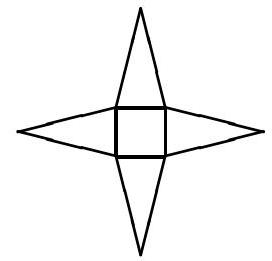
\includegraphics[max width=\textwidth, center]{2024_11_16_8518088a6e381b1443b2g-3}

\section*{PRACA KONTROLNA nr 4}
styczeń 2005r.

\begin{enumerate}
  \item Krawędzie oraz przekątna prostopadłościanu tworzą cztery kolejne wyrazy ciągu arytmetycznego, przy czym przekątna ma długość 7 cm . Jaką najkrótszą drogę musi przebyć mucha, aby wędrując po krawędziach tego prostopadłościanu odwiedziła wszystkie jego wierzchołki.
  \item Dany jest wielomian $w(x)=x^{4}-2 x^{2}-x+2$. Rozłożyć na czynniki możliwie najniższego stopnia wielomian $p(x)=w(x+1)-w(x)$.
  \item Na rysunku obok przedstawiono fragment mapy w skali 1:25000, który zawiera obszar lasu $L$ ograniczony czterema drogami. Na mapę jest naniesiona siatka kilometrowa, a dodatkowo umieszczono na niej układ współrzędnych pokrywający się z wybranymi liniami siatki. Zapisać obszar $L$ w postaci układu nierówności liniowych (w skali mapy). Obliczyć rzeczywiste pole obszaru $L$ wyrażając go w hektarach.\\
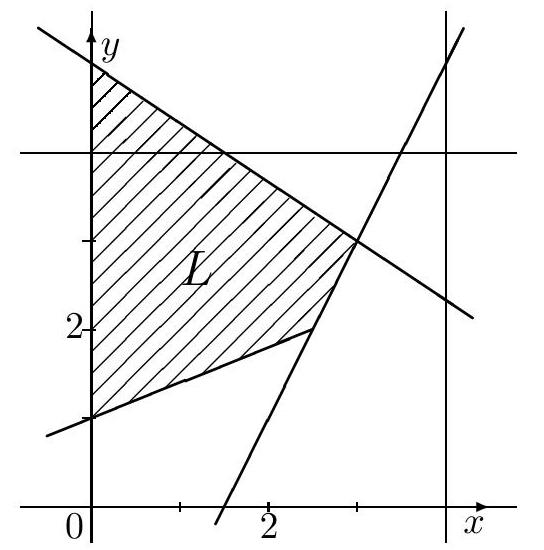
\includegraphics[max width=\textwidth, center]{2024_11_16_8518088a6e381b1443b2g-4}
  \item Na ile sposobów może Krzyś rozdzielić 12 jednakowych cukierków pomiędzy siebie i trójkę rodzeństwa, jeśli każdy ma otrzymać co najmniej dwa cukierki.
  \item W stożek wpisano sześcian o krawędzi $a$. Rozwinięcie powierzchni bocznej stożka tworzy wycinek koła o kącie środkowym $120^{\circ}$. Obliczyć tangens kąta pod jakim tworzącą tego stożka widać ze środka sześcianu.
  \item W trójkącie $A B C$ dane są kąty $\alpha$ i $\beta$ przy podstawie $\overline{A B}$ oraz środkowa $C D=s$ podstawy. Obliczyć pole tego trójkąta.
  \item Rozwiązać równanie $3^{\sin x}+9^{\sin x}+27^{\sin x}+\ldots=\frac{\sqrt{3}+1}{2}$, którego lewa strona jest sumą nieskończonego ciągu geometrycznego.
  \item Stosując zasadę indukcji matematycznej udowodnić nierówność:
\end{enumerate}

$$
1-\sqrt{2}+\sqrt{3}-\ldots+\sqrt{2 n-1}>\sqrt{\frac{n}{2}}, n \geqslant 1
$$

\begin{enumerate}
  \setcounter{enumi}{8}
  \item Wyznaczyć wszystkie wartości parametru rzeczywistego $p$, dla których krzywe o równaniach $y=\sqrt[3]{x}, \quad y=x^{p}$ przecinają się w pewnym punkcie pod kątem $45^{0}$. Rozwiązanie zilustrować odpowiednim rysunkiem.
\end{enumerate}

\section*{PRACA KONTROLNA nr 5}
luty 2005r.

\begin{enumerate}
  \item Firma otrzymała zlecenie na wyprodukowanie 80000 sztuk pewnego wyrobu w terminie 60 dni. Każdy z 20 pracowników firmy może wykonać w ciągu dnia 50 sztuk tego wyrobu. Reszta zamówienia może być zrealizowana przez dotychczasową załoge, ale za dodatkową pracę należy zapłacić podwójnie. Można też zatrudnić pewną liczbę nowych pracowników, którzy otrzymają $80 \%$ wynagrodzenia stałych pracowników. Nowy pracownik może po 4 dniach szkolenia wykonać 26 sztuk wyrobów w pierwszym dniu i zwiększać wydajność o 1 sztukę dziennie aż do osiągnięcia 50 sztuk. Ilu nowych pracowników należałoby zatrudnić wybierając drugi wariant i który wariant jest korzystniejszy dla firmy?
  \item Wyznaczyć wszystkie liczby rzeczywiste $a$ i $b$, których iloczyn oraz różnica kwadratów są równe ich sumie.
  \item Dane są zbiory na płaszczyźnie $A=\{(x, y):(x+y)(y-2 x) \leqslant 0\}$ oraz $B=$ $\{(x, y): y(3-x) \geqslant x\}$. Zaznaczyć na rysunku zbiór $C=A \cap B$. Podać wszystkie punkty zbioru $C$, których obie współrzędne są liczbami naturalnymi.
  \item W czworokącie wypukłym $A B C D$ przekątne $\overrightarrow{A C}=[7,-1] \quad$ i $\quad \overrightarrow{B D}=[3,3]$ przecinają się w punkcie $O$ odległym o $\sqrt{8}$ od wierzchołków $C$ i $D$. Wyznaczyć wektory $\overrightarrow{A B}$ i $\overrightarrow{B C}$ oraz narysować ten czworokąt.
  \item Wazon w kształcie graniastosłupa prawidłowego trójkątnego o krawędzi podstawy 4 cm i wysokości 25 cm napełniono całkowicie wodą. Następnie wylano część wody przechylając wazon w taki sposób, że poziom wody na dwóch krawędziach bocznych znajdował się w odległości 4 cm i 3 cm od górnego brzegu wazonu. Jaką wysokość będzie miał słup wody w wazonie po ustawieniu go z powrotem w pozycji pionowej?
  \item Zbadać monotoniczność ciągu o wyrazie ogólnym
\end{enumerate}

$$
a_{n}=\frac{2^{n}+2^{n+1}+\ldots+2^{2 n+1}}{2+2^{3}+\ldots+2^{2 n+1}}
$$

\begin{enumerate}
  \setcounter{enumi}{6}
  \item Sporządzić wykres funkcji $f(x)=\sqrt{5 x-x^{2}}-2$ nie przeprowadzając badania jej przebiegu i podać nazwę otrzymanej krzywej. Na podstawie wykresu określić liczbę rozwiązań równania $\left|\sqrt{5 x-x^{2}}-2\right|=p$ w zależności od parametru rzeczywistego $p$.
  \item Wykazać, że równanie kwadratowe $3 x^{2}+4 x \sin \alpha-\cos 2 \alpha=0$ ma dla każdej wartości parametru $\alpha$ dwa różne pierwiastki rzeczywiste. Wyznaczyć wszystkie wartości parametru $\alpha \in[0,2 \pi]$, dla których suma odwrotności pierwiastków tego równania jest nieujemna.
  \item Wyznaczyć asymptoty, przedziały monotoniczności oraz ekstrema lokalne funkcji
\end{enumerate}

$$
f(x)=|x-2|+\frac{5 x-4}{2 x^{3}}
$$

\section*{PRACA KONTROLNA nr 6}
marzec 2005r.

\begin{enumerate}
  \item Suma cyfr liczby trzycyfrowej wynosi 9 . Cyfra setek jest równa $1 / 8$ liczby złożonej z dwu pozostałych cyfr, a cyfra jednostek jest także równa $1 / 8$ liczby złożonej z dwu pozostałych cyfr. Co to za liczba?
  \item Obliczyć $\operatorname{tg} \beta$, gdzie $\beta \in[0, \pi]$, wiedząc, że $\cos \beta=\sin \alpha+\cos \alpha$ oraz że $\operatorname{tg} \alpha=-\frac{3}{4}, \alpha \in[0, \pi]$. W której ćwiartce leży kąt $\alpha+\beta$ ? Odpowiedź uzasadnić nie wykonując obliczeń przybliżonych.
  \item Wyznaczyć równania wszystkich parabol przechodzących przez punkt $P(1, \sqrt{3})$, których wierzchołek i punkty przecięcia z osią $O x$ tworzą trójkąt równoboczny o polu $\sqrt{3}$. Sporządzić rysunek.
  \item Rzucamy trzy razy kostką do gry. Jakie jest prawdopodobieństwo, że wyniki kolejnych rzutów utworzą a) ciąg arytmetyczny; b) ciąg rosnący?
  \item Z punktu $P$ leżącego w odległości $R$ od powierzchni kuli o promieniu $R$ poprowadzono trzy półproste styczne do tej kuli tworzące kąt trójścienny o jednakowych kątach płaskich. Obliczyć cosinus kąta płaskiego tego trójścianu.
  \item Okrąg o promieniu $r$ przecina każde z ramion kąta ostrego $2 \gamma \mathrm{w}$ dwóch punktach w taki sposób, że wyznaczają one dwie cięciwy jednakowej długości, a czworokąt utworzony przez te cztery punkty ma największe pole. Obliczyć odległość środka okręgu od wierzchołka kąta?
  \item Rozwiązać nierówność
\end{enumerate}

$$
\log _{x} \frac{1-2 x}{2-x} \geqslant 1
$$

\begin{enumerate}
  \setcounter{enumi}{7}
  \item Wyznaczyć i narysować zbiór wszystkich punktów płaszczyzny, których suma odległości od osi $O x$ i od okręgu $x^{2}+(y-1)^{2}=1$ wynosi 2 .
  \item Dana jest funkcja $f(x)=\cos 2 x+\frac{2}{3} \sin x \cdot|\sin x|$. a) Korzystając z definicji uzasadnić, że $f^{\prime}(0)=0$ b) Znaleźć wszystkie punkty z przedziału $[-\pi, \pi]$, w których styczna do wykresu funkcji $f(x)$ jest równoległa do stycznej w punkcie $x=\frac{\pi}{4}$. Rozwiązanie zilustrować odpowiednim rysunkiem.
\end{enumerate}

\section*{PRACA KONTROLNA nr 7}
\begin{enumerate}
  \item Liczba czteroelementowych podzbiorów zbioru $A$ jest 11 razy większa od liczby jego podzbiorów dwuelementowych, a zbiór $B \subset A$ ma tyle samo podzbiorów czteroelementowych co dwuelementowych. Ile podzbiorów co najwyżej trzyelementowych ma zbiór $A \backslash B$ ?
  \item Reszta z dzielenia wielomianu $x^{3}+p x^{2}-x+q$ przez trójmian $(x+2)^{2}$ wynosi $(-x+1)$. Obliczyć pierwiastki tego wielomianu.
  \item Kula $\mathcal{K}$ jest styczna do wszystkich krawędzi czworościanu foremnego o objętości $64 \mathrm{~cm}^{3}$. Czworościan ten przecięto płaszczyzną równoległą do jednej ze ścian i styczną do kuli $\mathcal{K}$. Obliczyć objętość otrzymanego ostrosłupa ściętego.
  \item Znaleźć wszystkie wartości parametru $p$, dla których przedział [1, 2] jest zawarty w dziedzinie funkcji
\end{enumerate}

$$
f(x)=\frac{\sqrt{x^{2}-3 p x+2 p^{2}}}{\sqrt{x+p}}
$$

\begin{enumerate}
  \setcounter{enumi}{4}
  \item Ze zbioru liczb czterocyfrowych wylosowano (ze zwracaniem) 4 liczby. Obliczyć prawdopodobieństwo tego, że co najmniej dwie z wylosowanych liczb czytane od strony lewej do prawej lub od strony prawej do lewej są podzielne przez 4.
  \item Należy wykonać stolik o symetrycznym owalnym blacie, jak pokazano na rysunku obok,\\
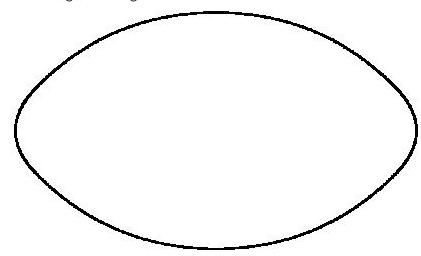
\includegraphics[max width=\textwidth, center]{2024_11_16_8518088a6e381b1443b2g-7}\\
o długości 1 m i szerokości 60 cm . Projektant przyjął, że brzeg blatu będzie się składał z czterech łuków okręgów, każdy o kącie środkowym $90^{\circ}$. Jakie powinny być promienie tych łuków, aby brzeg blatu był krzywą gładką? Podać powierzchnię blatu z dokładnością do $1 \mathrm{~cm}^{2}$.
  \item Styczna do okręgu $x^{2}+y^{2}-4 x-2 y-5=0 \mathrm{w}$ punkcie $A(-1,2)$, prosta $3 x+4 y-10=0$ oraz oś $O x$ tworzą trójkąt. Obliczyć jego pole i sporządzić rysunek.
  \item Rozwiązać równanie
\end{enumerate}

$$
\operatorname{ctg}^{2} x-\operatorname{ctg}^{4} x+\operatorname{ctg}^{6} x-\ldots=\frac{1+\cos 3 x}{2}
$$

którego lewa strona jest sumą nieskończonego ciągu geometrycznego.\\
9. Na walcu obrotowym o wysokości równej średnicy podstawy opisano ostrosłup prawidłowy trójkątny o najmniejszej objętości i taki, że jedna z podstaw walca leży na podstawie ostrosłupa. Obliczyć tangens kąta nachylenia ściany bocznej tego ostrosłupa do podstawy.


\end{document}